%!TEX root = Manuscrit.tex
\chapter{Généralisation}
\label{chap:generalisation}
\citationChap{I see no limit to the capabilities of machines. As microchips get smaller and faster, I can see them getting better than we are. I can visualize a time in the future when we will be to robots as dogs are to humans.}{Claude Shannon}
\minitoc

\chapsummary{%

}

\newpage

\section{Génération de données synthétiques}

Comme nous l'avons vu dans le~\cref{chap:extension}, il existe relativement peu de jeux de données annotés en imagerie hyperspectrale et ceux disponibles sont de petite taille. La difficulté d'annotation mais aussi la faible résolution spatiale des capteurs rend en effet complexe la constitution de jeux de données massifs. Des bases de spectres mesurés en laboratoire, comme celle de l'\gls{USGS}\footnote{\emph{USGS Spectral Library}: \url{https://speclab.cr.usgs.gov/spectral-lib.html}}, sont en pratique difficilement exploitable compte-tenu des différences de capteur, de calibration et de conditions d'acquisition. Il semble de ce fait pertinent de s'interroger sur les possibilités offertes par l'augmentation de données pour la classification de spectres.

L'augmentation de données consiste à introduire des échantillons synthétiques afin d'enrichir un jeu d'apprentissage~\cite{dyk_art_2012}. Cette pratique est particulièrement courante pour l'entraînement des \gls{CNN} depuis l'article séminal de~\citet{krizhevsky_imagenet_2012} afin d'éviter le surapprentissage. Dans un contexte de classification de données hyperspectrales, la rareté des échantillons annotés rend l'augmentation de données d'autant plus attrayante. Cependant, la plupart des travaux de l'état de l'art appliquant des \gls{CNN} 2D ou 3D à la classification de telles images~\cite{chen_deep_2016,makantasis_deep_2015,slavkovikj_hyperspectral_2015,lee_contextual_2016} se sont limités à des jeux de données de taille restreinte, ne permettant pas d'exploiter au mieux les capacités d'apprentissage de représentation offertes par les réseaux profonds.

Ainsi, quelques études se sont penchées sur l'enrichissement artificiel des jeux de données hyperspectraux mis à la disposition de la communauté. \citet{windrim_hyperspectral_2016} ont proposé un modèle physique permettant de simuler les déformations d'un spectre s'il était soumis à des conditions d'illumination différentes de celle de l'acquisition originale, ce qui leur permet d'introduire une invariance à ces changements environnementaux. Toutefois, cela nécessite la conception et la mise en \oe{}uvre d'un modèle physique expert qui n'est pas générique, introduisant une phase d'estimation de l'illumination pouvant être imprécise dans des images de télédétection. Plus simplement, \citet{chen_deep_2016} augmentent le nombre d'échantillons disponibles en générant des combinaisons linéaires des spectres existants et en ajoutant du bruit gaussien, en supposant ces altérations plausibles. Enfin, \citet{acquarelli_convolutional_2017} proposent de propager les annotations d'un pixel à ses voisins par \emph{clustering} afin d'incorporer des pixels observés mais initialement non annotés dans le jeu d'apprentissage. Si cette approche permet en effet d'apprendre à partir de pixels supplémentaires, le nombre total d'échantillons est toutefois borné par la taille de l'image acquise.

Ainsi, nous introduisons la problématique suivante: comment enrichir les bases d'apprentissage lorsque aucun \emph{a priori} physique n'est disponible, en ajoutant autant de nouveaux échantillons que désiré ? Une première piste de réponse se trouve dans les travaux de \citet{gemp_inverting_2017}. Ceux-ci implémentent des autoencodeurs variationnels qu'ils utilisent comme modèles génératifs pour le démélange de spectres, afin de déterminer les \emph{endmembers} d'une image. Pour la classification,~\citet{davari_gmm-based_2018} entraînent un \gls{GMM} afin d'estimer la distribution des caractéristiques spectrales après extraction des profils d'attributs. Ils peuvent ensuite générer de nouveaux vecteurs d'attributs synthétiques à partir de la distribution estimée, qui viennent enrichir le jeu d'apprentissage original.

Les modèles génératifs permettent en effet d'approximer les paramètres d'une distribution statistique latente à un ensemble d'observations pour en échantillonner de nouvelles. Nous proposons donc d’utiliser des modèles génératifs pour approximer la distribution latente des spectres au sein d'une image hyperspectrale afin de synthétiser de nouveaux échantillons susceptible d'appartenir à celle-ci. Il s'agit d'une approche ancrée uniquement dans les données, ne nécessitant aucun \emph{a priori} physique ni modèle de capteur.

En particulier, nous proposons d'utiliser les \glspl{GAN}~\cite{goodfellow_generative_2014} afin d'estimer la distribution des spectres de l'image, puis de générer de nouveaux spectres dont la présence dans la distribution réelle est statistiquement plausible. Afin de maximiser la quantité d'information exploitable, cette méthode se veut semi-supervisée afin de bénéficier aussi bien de la connaissance des spectres annotés que des spectres non-annotés. Nous validons l'intérêt d'utiliser ces spectres artificiels pour l'augmentation de données sur plusieurs jeux de données hyperspectraux publics, aériens comme satellitaires, sur différentes zones géographiques.

\subsection{Modèles génératifs adversaires}

\begin{figure}
		\resizebox{\textwidth}{!}{\begin{tikzpicture}
\usetikzlibrary{shapes.geometric}

\def \xgen {0}
\def \wblock {2}
\def \xdis {8}
\def \h {4}
\def \ydis {2}

\definecolor{blue}{RGB}{105, 150, 156}
\definecolor{red}{RGB}{170, 65, 57}
\definecolor{green}{RGB}{43, 130, 58}
\definecolor{orange}{RGB}{170, 111, 57}

% Générateur
\node [draw,trapezium, trapezium angle=75, shape border rotate=90,fill=blue!90!white, minimum width=3cm] (generator) at (1, 0) {\Large G};

% Discriminateur
\node [draw,trapezium, trapezium angle=75, shape border rotate=270,fill=green!50!white, minimum width=3cm] (discriminator) at (9, 2) {\Large D};
\node at (11.5, 2) (loss) {\small Réel/synthétique};
\draw[->,thick] (discriminator.east) -- (loss.west);

\node [draw,trapezium, trapezium angle=75, shape border rotate=270,fill=green!50!white, minimum width=3cm] (classifier) at (9, -2) {\Large C};
\node at (11.5, -2) (classes) {\small Classes};
\draw[->,thick,dashed] (classifier.east) -- (classes.west);
% Classifieur

% Bruit z
\node[rectangle, draw, rounded corners=6,fill=purple!50!white,minimum height=2.6cm] at (-1,1) (noise) {z};
\draw[->,thick,blue] (noise.east) to [bend right, out=0,in=-150] (generator.west);
% Condition
\node[rectangle, draw, rounded corners=6,fill=brown!50!white,minimum height=1cm] at (-1,-1) (condition) {c};
\draw[->,thick,blue] (condition.east) to [bend left, out=0,in=150] (generator.west);

% Spectres générés
\node[label={south:\footnotesize Spectres synthétiques}] at (\xgen+\wblock+2,0) (fake) {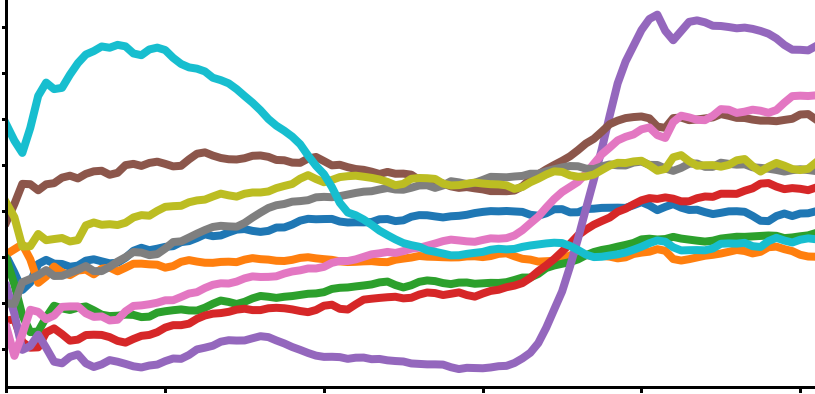
\includegraphics[width=2.5cm]{spectrum.png}};
\draw[->,thick,blue] (generator.east) -- (fake.west);
\draw[->,thick,blue] (fake.east) to [bend left=45,out=-25,in=-200] (discriminator.south west);
\draw [->, thick,blue,dashed] (fake.east) to [bend right=45,out=25,in=200] (classifier.north west) ;
% Jeu de données
\node [rectangle,draw,rounded corners=10, minimum width=3cm, minimum height=1cm,fill=gray!30!white] (unsupervised) at (4, 2) {\scriptsize Spectres non-étiquettés};
\node [rectangle,draw,rounded corners=10, minimum width=3cm, minimum height=1cm,fill=gray!30!white] (supervised) at (4, -2) {\scriptsize Spectres étiquettés};


\draw [->, thick,red] (unsupervised.east) -- node[above] {\footnotesize Spectres réels} (discriminator.west);
\draw [->, thick,red, dashed] (supervised.east) -- node[below] {\footnotesize Spectres réels} (classifier.west);
\draw [->, thick,red,dashed] (supervised.south) to [bend right=45, in=235] node[above] {\footnotesize Annotations} (classes.south west);
\draw [->, thick, blue,dashed] (condition.east) to [bend right=30, in=228] (classes.south);
\end{tikzpicture}
}
    \caption[La structure de \glsname{GAN} utilisée pour la synthèse de spectres artificiels.]{La structure du \glsname{GAN} utilisé pour la synthèse de spectres artificiels. Les flèches en \textcolor{BrickRed}{rouge} indiquent l'entraînement du classifieur et du discriminateur, tandis que les flèches en \textcolor{NavyBlue}{bleu} indiquent l'entraînement du générateur. Les flèches en pointillé indiquent les connexions qui ne sont utilisées que dans le cadre supervisé.}
    \label{fig:gan}
\end{figure}

Le principe des \glspl{GAN} a été introduit par~\citet{goodfellow_generative_2014} en 2014. L'idée est d'utiliser des réseaux de neurones profonds pour approximer la distribution statistique sous-jacente à un ensemble d'observations. Un générateur est ainsi entraîné pour approcher la projection entre un espace latent de bruit gaussien vers la distribution empirique observée. Cependant, la distribution n'est observée que sur quelques échantillons et l'on souhaite utiliser le générateur pour créer de nouveaux échantillons probables.Pour ce faire, le générateur est entraîné pour approcher la distribution à l'aide d'une fonction objectif adversaire. Cette fonction est implicitement définie en introduisant un second réseau, appelé discriminateur ou critique. Le discriminateur apprend à estimer si un échantillon provient de l'ensemble des données réelles ou bien a été généré artificiellement. À chaque étape de l'optimisation, le discriminateur est entraîné sur quelques itérations afin de lui permettre d'estimer la frontière entre données réelles et données synthétiques. Le générateur est ensuite optimisé de telle sorte à ce qu'il \emph{piège} le discriminateur, c'est-à-dire que les échantillons synthétisés soient indistinguables des exemples réels du point de vue du critique (cf.~\cref{def:gan}).

Plusieurs variantes des \glspl{GAN} ont été proposées depuis leur introduction. Nous utilisons ici un générateur $G$ et un discriminateur $D$ sur le principe des Wasserstein \glspl{GAN}~\cite{arjovsky_wasserstein_2017} avec la régularisation de~\citet{gulrajani_improved_2017}, dont l'entraînement est prévu pour minimiser la distance de Wasserstein entre la distribution réelle et la distribution synthétique. Toutefois, ce mode de fonctionnement est non-supervisé, c'est-à-dire qu'il n'est possible que de générer de nouveaux échantillons sans contrôle sur leur classe. Il serait possible de créer un générateur pour chaque classe, mais cela serait coûteux en temps et en mémoire. Dans notre cas, nous souhaitons pouvoir \emph{conditionner} le générateur par rapport à la classe du spectre que nous souhaitons synthétiser. Nous utilisons ainsi un classifieur auxiliaire $C$~\cite{odena_conditional_2017} qui ajoute une contrainte supplémentaire lors de l'optimisation du générateur en s'assurant que les spectres générés sont bien classifiés dans la classe choisie.
L'architecture complète est détaillée dans la~\cref{fig:gan}. Si $G$ et $D$ peuvent être entraînés sans annotation, c'est-à-dire de façon non-supervisée, $C$ doit être entraîné sur des exemples étiquetés. L'ensemble est donc semi-supervisé et peut exploiter simultanément les échantillons annotés et non-annotés sur l'ensemble de l'hypercube.

\begin{definition}
	\label{def:gan}
	Algorithme d'entraînement de réseaux de neurones génératifs adversaires:

	Avec $n$ la taille du \emph{batch}, $Z$ la distribution latente, $\Omega$ l'ensemble des échantillons (annotés ou non), $\Omega^* \subset \Omega$ le sous-ensemble des éléments annotés et $\mathcal{L}$ l'entropie croisée.
	Tant que le critère de convergence n'est pas atteint:
	\begin{enumerate}
		\item Optimisation de $D$. Répéter $k_D$ fois:
		\begin{itemize}
			\item Tirer aléatoirement un vecteur $z$ de $n$ éléments dans $\Omega$
			\item Itérer la descente de gradient sur $D$ pour maximiser $D(x)$
			\item Tirer aléatoirement un vecteur $z$ de $n$ éléments dans $Z$
			\item Itérer la descente de gradient sur $D$ pour minimiser $D(G(z))$
		\end{itemize}
		\item (facultatif) Optimisation de $C$. Répéter $k_C$ fois:
		\begin{itemize}
			\item Tirer aléatoirement un vecteur $x^*$ de $n$ éléments dans $\Omega^*$, avec $y$ le vecteur de classes
			\item Itérer la descente de gradient sur $C$ pour minimiser $\mathcal{L}(C(x^*),y)$
		\end{itemize}
		\item Optimisation de $G$.
		\begin{itemize}
			\item Tirer aléatoirement un vecteur $z$ de $n$ éléments dans $Z$
			\item (facultatif) Générer et concaténer à $z$ son vecteur de condition $c$
			\item Générer les échantillons $\hat{x} = G(z)$
			\item Calculer la fonction de coût $\mathcal{L}_\mathit{totale}(z) = -D(\hat{x})$
			\item (facultatif) Ajouter l'erreur sur $C$ : $\mathcal{L}_\mathit{totale}(z) := \mathcal{L}_\mathit{totale}(z) + \mathcal{L}(C(\hat(x),c))$
			\item Itérer la descente de gradient sur $G$ pour minimiser $\mathcal{L}_\mathit{totale}$
		\end{itemize}
	\end{enumerate}
\end{definition}

\subsection{Cadre expérimental}
\label{sec:experimental_setup}

Nous entraînons ce \glspl{GAN} sur les jeux de données Pavia University, Pavia Center, Indian Pines et Botswana (cf.~\cref{sec:hyperspectral_datasets}) en utilisant les réflectances corrigées atmosphériquement lorsqu'elles sont disponibles. Comme nous essayons de générer des spectres individuels et non des hypercubes, nous utilisons pour $G$, $D$ et $C$ des réseaux simples, entièrement connectés à 4 couches, utilisant la fonction d'activation \emph{Leaky \gls{ReLU}}~\cite{maas_rectifier_2013}. L'intérêt d'une telle fonction d'activation par rapport à la \gls{ReLU} usuelle est d'avoir un gradient non-nul sur toute sa plage de fonctionnement, ce qui facilite la rétropropagation du gradient de $D$ vers $C$. La sortie de $G$ est suivie par une sigmoïde pour contraindre les valeurs de réflectance synthétisée entre $0$ et $1$. $D$ ne possède qu'une seule sortie et $C$ possède autant de sorties que le jeu de données a de classes.

L'optimisation des trois réseaux se fait en utilisant la politique de descente de gradient stochastique \emph{RMSProp}~\cite{tielman_lecture_2012}. L'ensemble est entraîné durant \num{100000} itérations avec une taille de \emph{batch} de 256, $C$ et $D$ étant entraînés 2 fois à chaque itération.

Par ailleurs, il apparaît nécessaire d'établir une performance de référence afin d'évaluer la pertinence des \glspl{GAN} pour la synthèse de spectres. Nous implémentons donc un modèle de mélange gaussien en utilisant la bibliothèque scikit-learn~\cite{pedregosa_scikit-learn_2011}. Nous reconstruisons un mélange pour chaque classe du jeu de données utilisant 10 composantes, que nous utilisons par la suite pour générer de nouveaux spectres.

\subsection{Analyse des spectres générés}
\label{sec:analysis}

Dans un premier temps, nous cherchons à comparer selon plusieurs critères les distributions synthétiques et réelles. Pour ce faire, nous entraînons d'abord deux \glspl{GAN} sur Pavia University et Indian Pines.

\begin{figure}
\begin{subfigure}{0.5\textwidth}
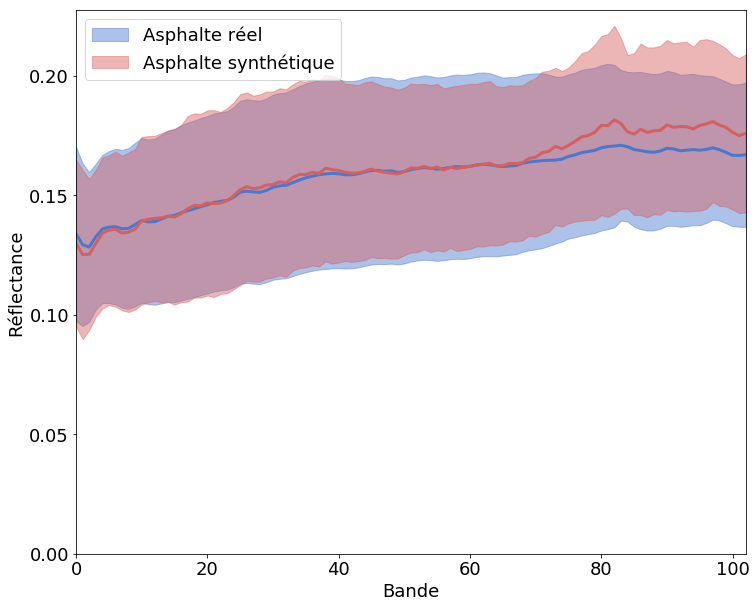
\includegraphics[width=\textwidth]{asphalt_spectra_fr}
\end{subfigure}%
\begin{subfigure}{0.5\textwidth}
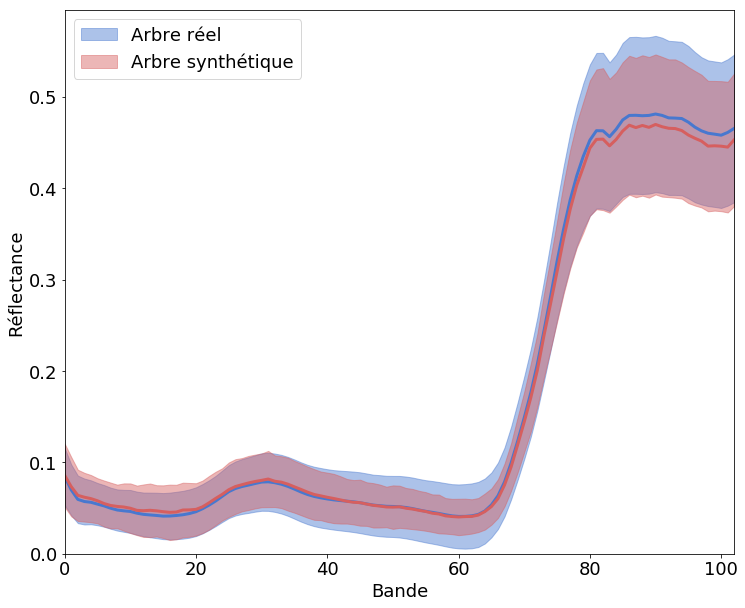
\includegraphics[width=\textwidth]{trees_spectra_fr}
\end{subfigure}
\caption{Spectre moyen et écart-type pour deux classes de matériaux du jeu de données Pavia Center. Les échantillons synthétiques moyens sont plus bruités et sont surappris sur certaines propriétés spectrales locales.}
\label{fig:mean_spectra}
\end{figure}

Visuellement, il est possible de constater dans la~\cref{fig:mean_spectra} que les spectres générés présentent des moments statistiques très similaires aux spectres réels. Les formes globales des spectres sont correctement approchées pour chaque classe. Toutefois, deux points négatifs sont identifiables. Tout d'abord, les spectres synthétiques moyens semblent plus bruités que leurs équivalents réels, ce qui signifie que le \gls{GAN} a surappris certaines particularités liées aux échantillons d'entraînement choisis. En outre, l'écart-type de la distribution synthétique est inférieur à celui de la distribution réelle, ce qui signifie que les faux spectres sont moins diversifiés que les vrais. Ces deux constatations indiquent que le générateur souffre partiellement d'une forme d'apprentissage appelée \emph{mode collapse}~\cite{salimans_improved_2016}.

\begin{figure}[t]
\begin{subfigure}{\textwidth}
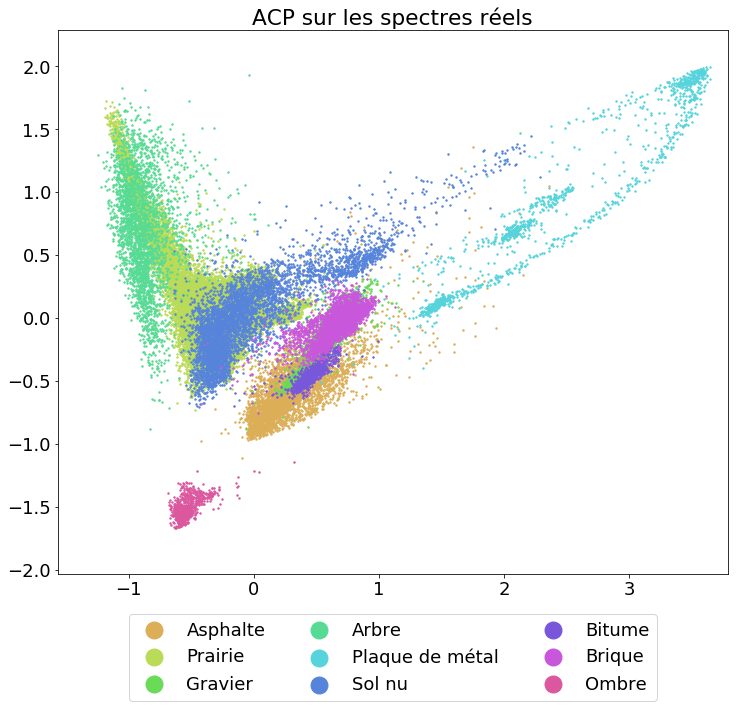
\includegraphics[width=0.5\textwidth]{pca_paviau_real_fr}%
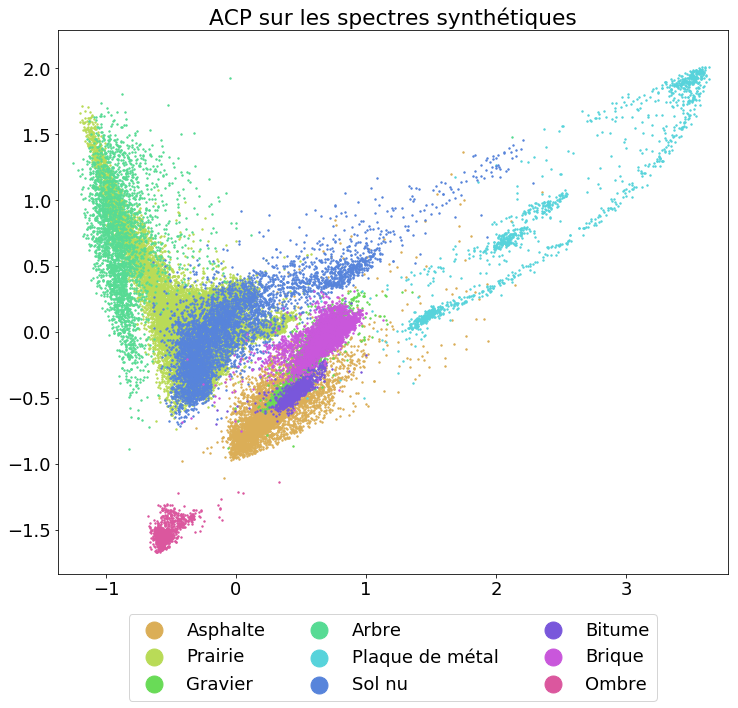
\includegraphics[width=0.5\textwidth]{pca_paviau_fake_fr}%
\caption{Pavia University}
\end{subfigure}
\begin{subfigure}{\textwidth}
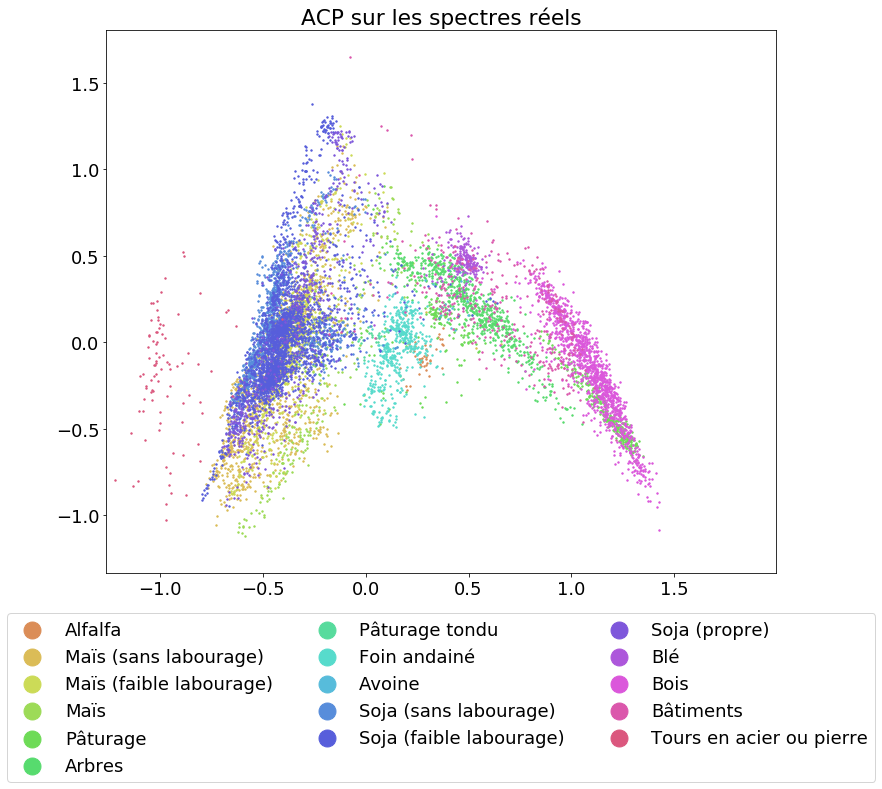
\includegraphics[width=0.5\textwidth]{pca_ip_real_fr}%
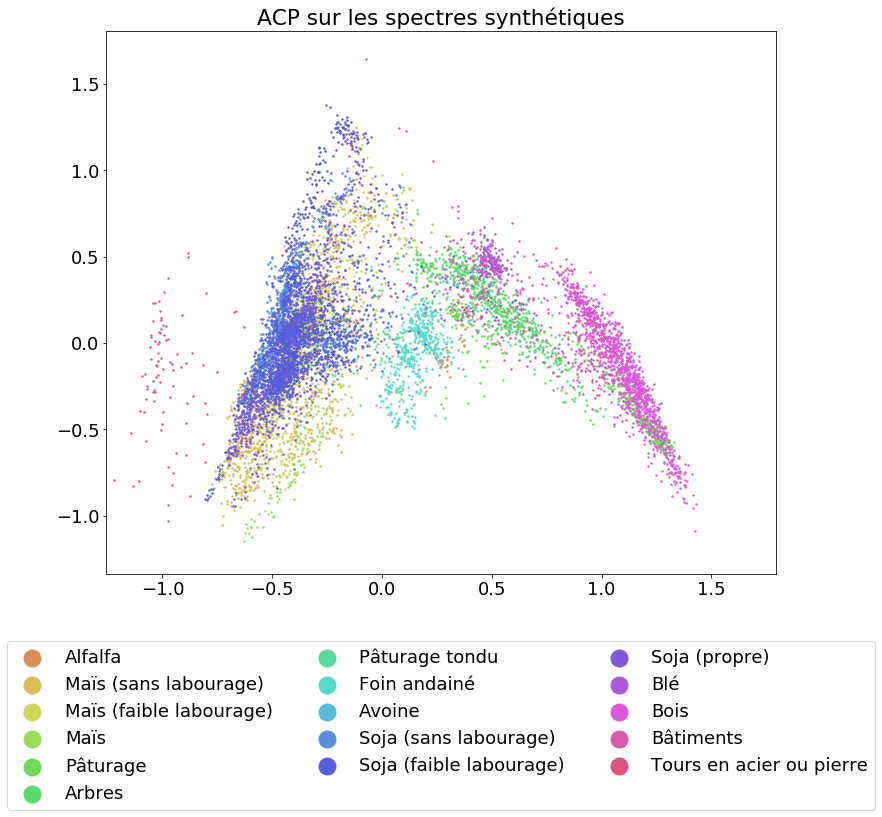
\includegraphics[width=0.5\textwidth]{pca_ip_fake_fr}%
\caption{Indian Pines}
\end{subfigure}
\caption[\glsname{ACP} sur les spectres réels et synthétiques.]{\glsname{ACP} sur les spectres réels et synthétiques. Les spectres réels correspondent à l'ensemble des échantillons annotés de l'image. Les deux ensemble contiennent le même nombre d'éléments.}
\label{fig:pca}
\end{figure}

Pour mieux comprendre l'impact de ce surapprentissage, nous appliquons une \gls{ACP} afin de projeter les spectres réels et synthétiques dans un espace de représentation à deux dimensions (cf.~\cref{fig:pca}). Les groupes formés par les différentes classes sont correctement reproduits par les échantillons synthétiques. Cependant, la distribution synthétique présente également quelques déformations montrant que, si le \gls{GAN} a bien réussi à modéliser la forme générale des différents types de spectres, il n'est cependant pas parvenu à reproduire l'ensemble de leurs spécificités.

\begin{table}[t]
	\begin{tabularx}{\textwidth}{c Y Y Y Y}
        Découpage & \multicolumn{2}{c}{Aléatoire (uniforme)} & \multicolumn{2}{c}{Disjoint}\\
        \toprule
		\textbf{Apprentissage $\backslash$ Test} & Réels & Synthétiques & Réels & Synthétiques\\
        \midrule
        %\textbf{Train} & & & &\\
        Réels & \num{89.5} & \num{98.3} & \num{87.2} & \num{98.8}\\
        Synthétiques & \num{87.8} & \num{99.2} & \num{79.4} & \num{99.9}\\
        \bottomrule
	\end{tabularx}
    \caption{Exactitudes d'une \glsname{SVM} linéaire appliquée sur les spectres réels et synthétiques du jeu de données Pavia University.}
    \label{table:svm_separation}
\end{table}

Nous pouvons essayer d'estimer comment la distribution synthétique respecte les frontières entre classes de la distribution réelle en entraînant une \gls{SVM} linéaire sur les spectres réels et en l'appliquant pour séparer les spectres synthétiques. La \gls{SVM} va calculer les meilleurs hyperplans séparateurs pour la véritable distribution. Idéalement, ces hyperplans devraient séparer les spectres synthétiques exactement de la même façon. S'ils séparent nettement moins bien les spectres synthétiques, alors cela signifie que le générateur créé des échantillons irréalistes. S'ils séparent nettement mieux les échantillons, alors le générateur créé des exemples synthétiques trop similaires entre eux et regroupés autour des centroïdes correspondant aux classes réelles. Les résultats sont détaillés dans le~\cref{table:svm_separation}. Nous considérons deux approches\,: entraînement sur 3\% des spectres tirés au hasard uniformément ou sur 50\% de l'image, disjoint spatialement de la zone de validation. Dans le mode non-supervisé, nous utilisons également les échantillons non-annotés. Comme attendu, la \gls{SVM} sépare plus facilement les échantillons synthétiques que les spectres réels. Toutefois, entraîner la \gls{SVM} sur les spectres synthétiques uniquement permet tout de même de séparer les spectres réels dans une certaine mesure. Autrement dit, si les échantillons synthétiques sont moins diversifiés que les spectres réels, ils sont néanmoins représentatifs des différentes classes, et ce alors même que ces spectres sont générés \emph{ex nihilo} à partir de bruit aléatoire.

\begin{figure}[ht]
\begin{subfigure}{\textwidth}
	\begin{subfigure}{0.5\textwidth}
		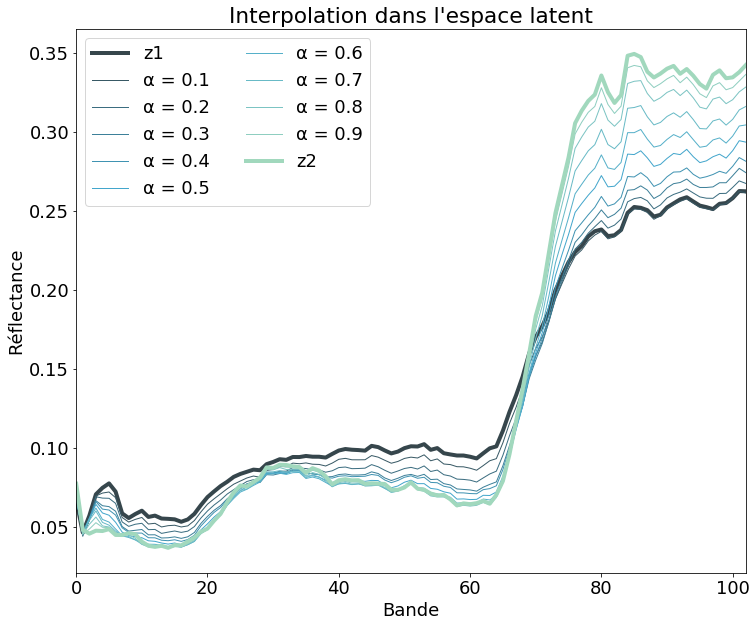
\includegraphics[width=\textwidth]{interpolation_intraclass_latent_fr}
	\end{subfigure}
	\begin{subfigure}{0.5\textwidth}
		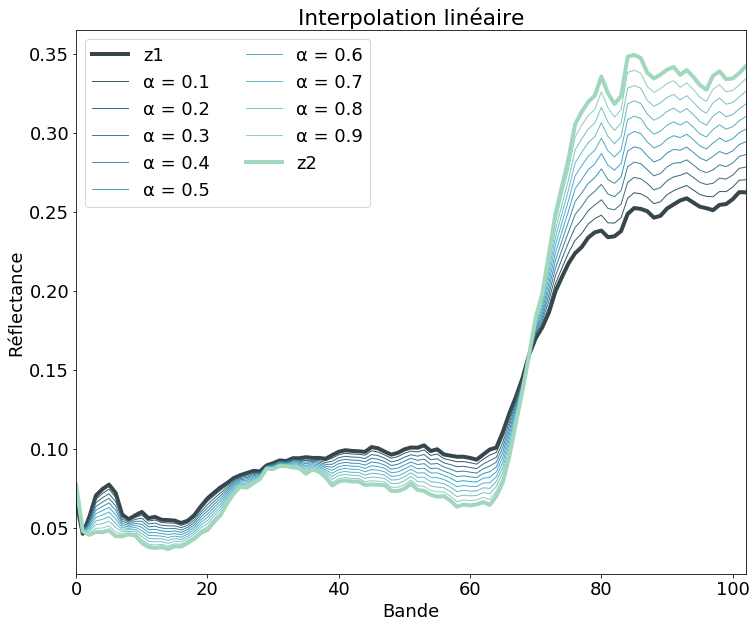
\includegraphics[width=\textwidth]{interpolation_intraclass_linear_fr}
	\end{subfigure}
	\caption{Interpolation entre deux vecteurs latents de la classe prairie.}
	\label{fig:interpolation_intra}
\end{subfigure}

\begin{subfigure}{\textwidth}
	\begin{subfigure}{0.5\textwidth}
		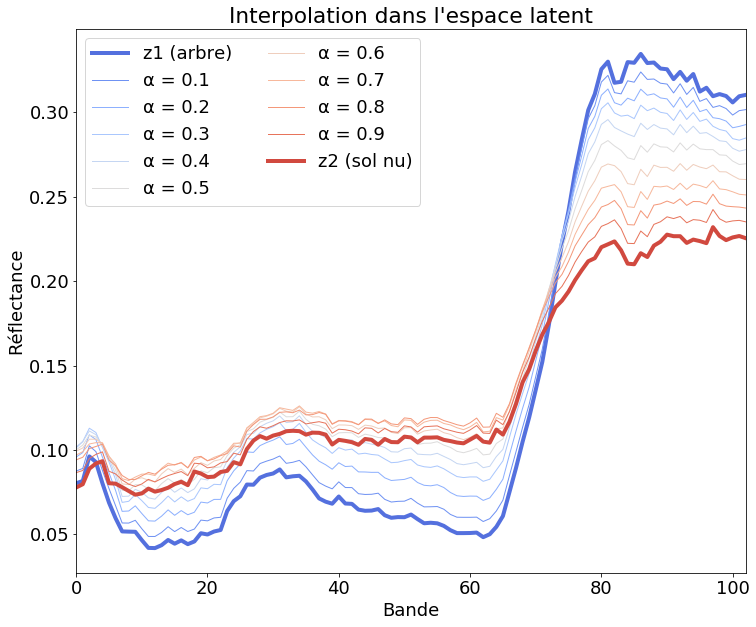
\includegraphics[width=\textwidth]{interpolation_interclass_latent_fr}
	\end{subfigure}
	\begin{subfigure}{0.5\textwidth}
		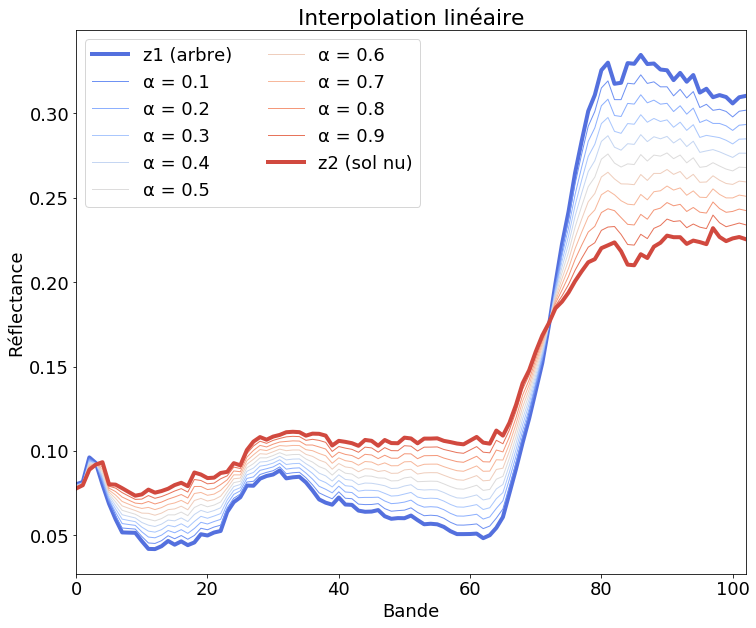
\includegraphics[width=\textwidth]{interpolation_interclass_linear_fr}
	\end{subfigure}
	\caption{Interpolation à vecteur latent constant entre les classes arbre et sol nu.}
	\label{fig:interpolation_inter}
\end{subfigure}

\caption{Interpoler entre différents vecteurs ou conditionnements de l'espace latent permet d'explorer la variété des spectres de façon continue. Le \glsname{GAN} est entraîné sur le jeu de données Pavia University. $\alpha$ contrôle l'interpolation.}
\label{fig:interpolation}
\end{figure}

Finalement, comme les \gls{GAN} permettent d'établir une projection entre un espace de représentation latent et le signal, il est possible d'explorer la variété des spectres en interpolant de façon continue entre deux points de l'espace latent. En effet, si $z_1$ et $z_2$ sont deux vecteurs aléatoires tirés dans la distribution gaussienne latente, alors il est possible d'interpoler entre les deux le long de l'hypersphère unité:
\begin{equation}
	\begin{cases}
		\forall \alpha \in [0,1],~~z_\alpha = \frac{\sin((1 - \alpha)\cdot \omega)}{\sin{\omega}} \cdot z_1 + \frac{\sin(\alpha \cdot \omega)}{\sin{\omega}} \cdot z_2\\
		\hat{x}_\alpha = G(z_\alpha, c) \text{ avec } x_0 = G(z_1, c) \text{ et } x_1 = G(z_2, c)
	\end{cases}
\end{equation}
avec $\omega$ l'angle entre $z_1$ et $z_2$. En particulier, il est également possible d'interpoler à vecteur de bruit fixe entre deux vecteurs de conditionnement $c_1$ et $c_2$:
\begin{equation}
	\begin{cases}
		\forall \alpha \in [0,1],~~c_\alpha = (1-\alpha) \cdot c_1 + \alpha \cdot c_2\\
		\hat{x}_\alpha = G(z, c_\alpha) \text{ avec } x_0 = G(z, c_1) \text{ et } x_1 = G(z, c_2)
	\end{cases}
\end{equation}

L'interpolation entre deux points de l'espace latent permet de générer une progression spectrale telle qu'illustrée par la~\cref{fig:interpolation_intra}. En comparaison à une interpolation linéaire directement effectuée entre les deux signatures spectrales, les échantillons générés ne sont pas régulièrement espacés car le chemin dans l'espace latent encode un réalité un chemin sur la \emph{variété} des spectres. Calculer entre un barycentre entre les deux vecteurs représentant les réponses spectrales n'a pas nécessairement de sens physique, car le vecteur qui en résulte n'est pas nécessairement sur la variété des spectres réels. À l'inverse, les interpolations générées par le \gls{GAN} approchent fidèlement le chemin sur la variété qui relie les deux extrémités.

De la même façon, il est possible de générer des mélanges de spectres en interpolant entre les vecteurs de conditionnement, ce qui est illustré par la~\cref{fig:interpolation_inter}. Les mélanges de matériaux en condition réels présentent souvent des propriétés non-linéaires causées par la géométrie du terrain ou des effets de réflexion et d'occlusion. Ici encore, le \gls{GAN} génère des échantillons dont la présence sur la variété des spectres réels est plausible, tandis que l'interpolation linéaire parcourt un espace arbitraire. Si l'on considère que les mélanges produits par le générateur sont réalistes, alors celui-ci effectue l'inverse de l'opération de démélange. Une approche d'apprentissage par dictionnaire, par inversion de modèle~\cite{gemp_inverting_2017} ou par plus proche voisin pourrait alors permettre, à partir d'un spectre réel soupçonné d'être un mélange, de revenir à ses \emph{endmembers} par une cartographie exhaustive de l'espace latent.

\subsection{Augmentation de données}
\label{sec:augmentation}

\begin{table}[!t]
	\setlength\tabcolsep{3pt}
	\begin{tabularx}{\textwidth}{c Y Y Y Y Y Y Y Y}
	\toprule
    Jeu de données & \multicolumn{2}{c}{Pavia University} & \multicolumn{2}{c}{Pavia Center} & \multicolumn{2}{c}{Botswana} & \multicolumn{2}{c}{Indian Pines}\\
    Augmentation & 3\% (r) & 50\% (s) & 3\% (r) & 50\% (s) & 3\% (r) & 50\% (s) & 3\% (r) & 50\% (s)\\
    \midrule
    $\emptyset$ & \num{92.72} & \num{86.22} & \num{98.93} & \num{96.26} & \num{86.90} & \num{84.87} & \num{79.44} & \num{74.00}\\
    GAN & \num{92.95} & \num{86.47} & \num{99.00} & \num{96.26} & \num{87.72} & \num{84.60} & \num{80.01} & \num{74.81}\\
    ss-GAN & \num{93.12} & \num{87.20} & \num{98.93} & \num{96.70} & \num{88.40} & \num{85.27} & \num{80.42} & \num{74.58}\\
%     \midrule
%     \multirow{4}{*}{CNN 1D} & $\emptyset$ & - & - & - & - & - & - & - & -\\
%     & GAN & - & - & - & - & - & - & - & -\\
%     & ss-GAN & - & - & - & - & - & - & - & -\\
    \bottomrule
    \end{tabularx}
    \caption{Scores d'exactitudes obtenues par un classifieur entièrement connecté à 4 couches sur plusieurs jeux de données en utilisant différentes augmentations de données. Le partage du jeu de données se fait en coupant l'image en deux (s) ou par un échantillonnage aléatoire uniforme de 3\% des pixels annotés (r).}
    \label{table:da_results}
\end{table}

Les échantillons générés étant plausibles et représentatifs des spectres réels, nous suggérons de les utiliser pour enrichir les jeux de données annotés pré-existants. Nous testons cette idée sur plusieurs jeux de données : Indian Pines (aérien, rural), Pavia University (aérien, péri-urbain), Pavia Center (aérien, urbain) et Botswana (satellite, rural). Les résultats en mode supervisé et semi-supervisé sont détaillés dans le~\cref{table:da_results}. Augmenter le jeu de données à l'aide des faux spectres permet de légèrement augmenter les performances du classifieur.

Toutefois, augmenter drastiquement le nombre de faux spectres n'améliore pas plus la classification et finit même par la dégrader. En effet, dans ce cas les échantillons synthétiques deviennent prédominants dans la fonction de coût et dégradent les performances du classifieur, le ramenant vers le cas de la \gls{SVM} entraînée uniquement sur les faux spectres.

Dans l'absolu, la mise en \oe{}uvre de \glspl{GAN} pour la génération de spectres \emph{ex nihilo} et l'augmentation de données n'apporte que des bénéfices légers. Notamment, les \glspl{GAN} ne peuvent qu'approcher la distribution des spectres réellement observés et d'interpoler à l'intérieur de celle-ci, mais peuvent difficilement générer des nouvelles observations à l'extérieur de la distribution. Puisque la classification consiste à déterminer les frontières entre classes, ce sont donc les échantillons éloignés des centroïdes qui sont les plus informatifs. Ainsi, l'approche semi-supervisée permet de générer des spectres annotés présentant des propriétés statistiques proches des observations non-annotées, et donc d'augmenter la quantité d'information disponible au classifieur, mais l'approche supervisée pure est rapidement limitée. Toutefois, cela a permis de démontrer la capacité des \glspl{GAN} à modéliser des distributions statistiques complexes sans aucune connaissance physique. Cette conclusion devient particulièrement intéressante lorsque l'on considère les efforts passés et actuels investis dans la développement de simulateurs de données hyperspectrales~\cite{borner_sensor_2001}. Ceux-ci utilisent d'une part les mesures en laboratoire des réflectances de matériaux connus et d'autre part des modèles physiques de capteur et d'atmosphère. Cependant, les modèles introduisent nécessairement des approximations et des simplifications qui ne permettent pas de tenir compte des effets optiques, atmosphériques et électroniques les plus complexes (bruit provoqué par la chauffe des composants, rayons lumineux parasitaires, turbulences\dots). Une combinaison mêlant approche statistique et physique serait de conditionner les \glspl{GAN} par les spectres produits par ces simulateurs, pour laisser au générateur le soin de modéliser ces phénomènes complexes, afin de rendre les spectres simulés réalistes et de les aligner avec les acquisitions réelles.

\section{Cas des données massives}

\subsection{Diversité des scènes}

Jusqu'à présent, nous nous sommes intéressés à des jeux de données ne couvrant qu'une seule scène. En effet, les expériences des~\cref{chap:cartographie,chap:extension,chap:multimodal} ont été effectuées sur les villes de Vaihingen et Potsdam, pour une seule ville à la fois. Néanmoins, cela ne correspond pas à un cas applicatif réel. L'observation de la Terre passe par la répétition des acquisitions sur l'ensemble du globe. Par conséquent, il est nécessaire d'évaluer les capacités de généralisation des modèles mis en \oe{}uvre dans un cadre géographique varié. Une question naturelle est de savoir comment se comportent les réseaux profonds sur de nouvelles acquisitions. S'il est possible de s'attendre à une dégradation des performances prédictives des modèles, compte-tenu du surapprentissage inhérent à l'entraînement sur une seule scène, il est important d'être en mesure de la quantifier.

Pour ce faire, nous étudions tout d'abord les transferts entre deux scènes similaires: \gls{ISPRS} Potsdam et \gls{ISPRS} Vaihingen. Les deux jeux de données sont constitués d'images aériennes \gls{THR} recouvrant les canaux \gls{IRRV} acquises en zone urbaine et ont été annotés pour les mêmes classes d'intérêt. Les villes présentent néanmoins des caractéristiques différentes: Potsdam est six fois plus peuplée que Vaihingen pour une densité de population deux fois plus élevée. Les architectures des bâtiments sont différentes, tout comme l'agencement urbain. En première approche, nous considérons le réseau SegNet entraîné sur les images \gls{IRRV} de Potsdam au~\cref{chap:cartographie}, que nous appliquons tel quel sur une image de Vaihingen. Les cartes générées sont présentés dans la~\cref{fig:potsdam_transfert}. Dans l'ensemble, les grandes composantes de l'image sont retrouvées par le réseau, en particulier les routes et les bâtiments. Néanmoins, on peut constater d'une part une importance confusion des bâtiments avec la classe de rejet (en rouge) mais aussi l'absence de voiture. Cette dernière observation s'explique par la différence de résolution entre les deux jeux de données. Le modèle entraîné sur Potsdam a optimisé ses filtres pour une image à \SI{5}{\centi\meter/\px} et est ensuite appliqué sur une image de Vaihingen à \SI{9}{\centi\meter/\px}. Le facteur d'échelle ayant changé, les véhicules sont alors plus petits qu'attendus et deviennent invisibles. Dans l'ensemble, l'exactitude de la prédiction sur Vaihingen par un modèle entraîné uniquement sur Potsdam est de 77\%, ce qui est nettement inférieur aux résultats que nous avions présenté dans le~\cref{chap:cartographie}. Entraîner un modèle sur une scène unique semble donc biaiser celui-ci, au détriment de son applicabilité à de nouvelles acquisitions.

\missingfigure{Tuile de Vaihingen classifiée par SegNet(Potsdam) et SegNet(Vaihingen)}

Une alternative réaliste consisterait alors à annoter une faible partie des données cible (ici, Vaihingen) et de réaliser un \emph{fine-tuning} du modèle entraîné sur Potsdam. Cela permettrait au modèle d'ajuster ses poids pour tenir compte des nouvelles images sans pour autant entraîner un réseau en entier.

\missingfigure{Tableau : résultats sur Vaihingen avec 1/2 tuile, 1 tuile et toutes les tuiles (Javiera) vs. résultats sur Vaihingen mais préentraîné avec Potsdam sur 1/2 tuile, 1 tuile et toutes les tuiles}

\subsection{Passage à l'échelle}

Nous collectons un jeu de données à large échelle sur la France métropolitaine. Nous utilisons la BD ORTHO de l'\gls{IGN} comme source d'images aériennes à une résolution de \SI{50}{\centi\meter/\px}. Les annotations du projet Copernicus \emph{Urban Atlas} 2012 sont utilisées, en complément des données \emph{Open Data} du cadastre français. Nous considérons les images de la BD ORTHO de 2012 à 2014 sous licence \emph{open data}. Nous filtrons hors du cadastre les bâtiments ajoutés à la base de données après le 1\ier janvier 2013. 16 agglomérations font partie du jeu de données, que nous intitulons \emph{MiniFrance} (cf.~\cref{tab:minifrance,fig:minifrance}).

\begin{table}[h]
\caption{Liste des villes présentes dans MiniFrance.}
\label{tab:minifrance}
	\begin{tabularx}{\textwidth}{c Y Y Y}
	\toprule
	\emph{Conurbation} &  Nombre de tuiles &  \% pixels & Couleur \\
	\midrule
	Nice & 170 & \num{8.01}\% & \mybox{202,0,205} \\
	Nantes, Saint-Nazaire  & 226 & \num{10.65}\% & \mybox{111,204,240} \\
	Le Mans & 107 & \num{5.04}\% & \mybox{53,182,180}  \\
	Lorient & 68 & \num{3.20}\%  & \mybox{175,254,122} \\
	Brest & 88  & \num{4.14}\% &  \mybox{80,145,229}\\
	Caen & 126 & \num{5.94}\%  & \mybox{242,248,158}  \\
	Dunkerque, Calais, Boulogne-sur-Mer & 150 & \num{7.07}\% &  \mybox{157,205,24} \\
	Saint-Brieuc & 71 &  \num{3.34}\% &  \mybox{75,236,75}\\
	Marseille, Martigues & 162 & \num{7.63}\% &  \mybox{51,98,164}\\
	Rennes & 196 & \num{9.24}\% & \mybox{106,0,255} \\
	Angers & 123  & \num{5.79}\% & \mybox{131,70,136}\\
	Quimper & 79 & \num{3.72}\% & \mybox{217,116,218}\\
	Vannes & 73 & \num{3.44}\% & \mybox{171,65,168}\\
	Clermont-Ferrand & 150 & \num{7.07}\% & \mybox{26,93,83}\\
	Lille, Arras, Lens, Douai, Hénins & 275 & \num{12.96}\% & \mybox{195,57,149}\\
	Cherbourg & 57 & \num{2.68}\% & \mybox{249,191,30}\\ \bottomrule
	\end{tabularx}
\end{table}

Chaque tuile de la BD ORTHO est une image à \SI{50}{\centi\meter/\px} de dimensions \SI{10000x10000}{\px}. Les polygones issus des 28 classes de UrbanAtlas 2012 et les empreintes de bâtiments issues du cadastre sont rasterisées pour correspondre aux images.

\begin{figure}[h]
    \centering
    \begin{subfigure}[b]{0.3\textwidth}
        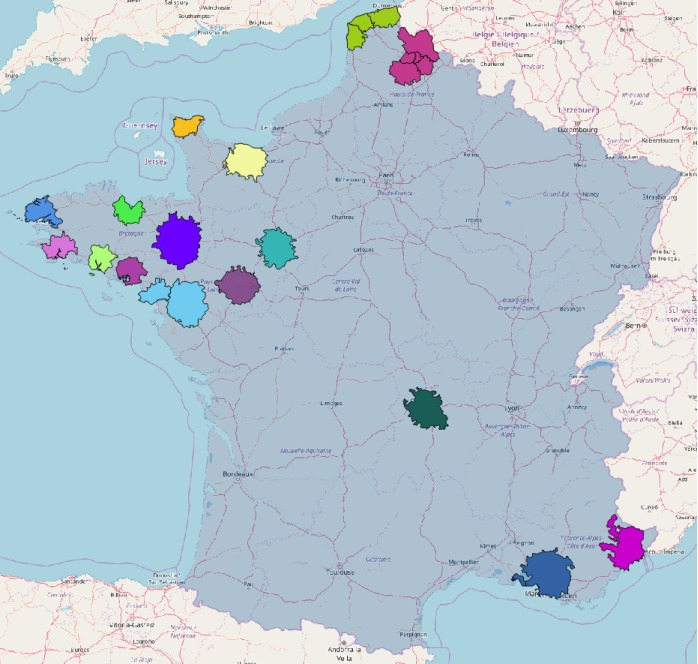
\includegraphics[width=\textwidth]{minifrance}
        \caption*{Répartition des villes}
    \end{subfigure}
    \begin{subfigure}[b]{0.28\textwidth}
        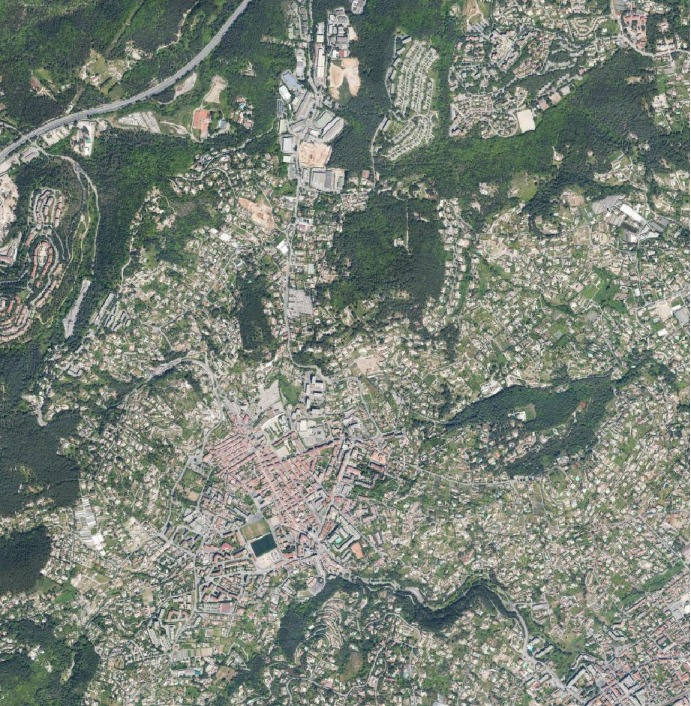
\includegraphics[width=\textwidth]{nice}
        \caption*{Ortho-image (Nice)}
    \end{subfigure}
    \begin{subfigure}[b]{0.28\textwidth}
        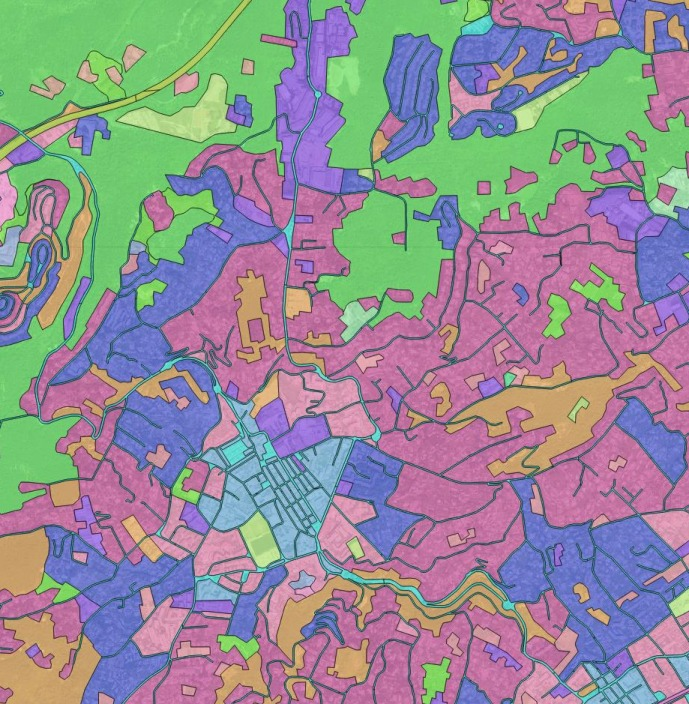
\includegraphics[width=\textwidth]{nice_gt}
        \caption*{Annotations (UrbanAtlas)}
    \end{subfigure}
       \caption{Présentation du jeu de données MiniFrance.}
			 \label{fig:minifrance}
\end{figure}

\missingfigure{Résultats 1\iere baseline sur MiniFrance (Javiera)}

%\bibliographystyle{plainnat}
%\bibliography{Chapitre5/Biblio}
\printbibliography[heading=subbibliography]
